\subsection{Eure Profs}
Um euch einen kleinen Vorgeschmack auf die Leute zu geben, die euch demn"achst mit ihrem Wissen begl"ucken wollen, seien sie hier kurz aufgef"uhrt:
\subsubsection{Algorithmen und Datenstrukturen}


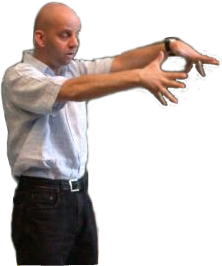
\includegraphics[width=0.7\linewidth]{bilder/dozenten/fekete_frei.png}\\
\textit{Prof. S\'andor Fekete}

Diese Vorlesung vermittelt Programmiersprachenunabh"angige Konzepte wie B"aume, Listen oder Stacks. Wer nicht wei"s, was sich hinter diesen Begriffen verbirgt, sollte auf keinen Fall die "Ubungen verpassen.

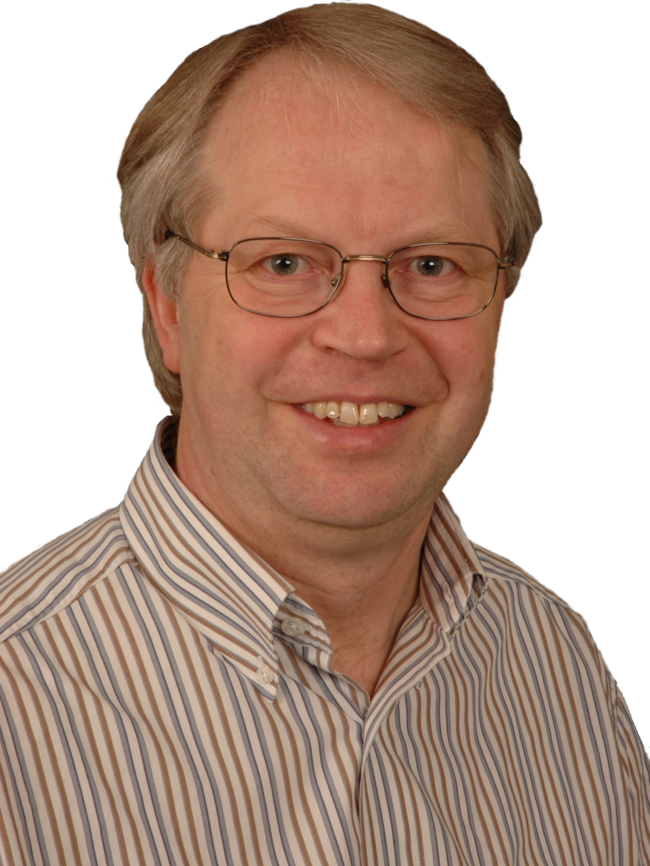
\includegraphics[width=0.6\linewidth]{bilder/dozenten/struck.png}\\
\textit{Dr. Werner Struckmann}

\subsubsection{Programmieren 1}

Programmiert wird hier fast ausschlie"slich in Java. Wer keine oder nur wenig Erfahrungen mit Java gemacht hat, sollte unbedingt die kleinen "Ubungen bearbeiten.
%Die Klausur ist ber"uhmt f"ur ihre hohe Durchfallquote! (Gl"ucklicherweise sind daran nicht die Informatiker schuld)
%Trotzdem: Programmieren ist das Handwerk der Informatik, also macht eurem Fach Ehre.

\subsubsection{Lineare Algebra}

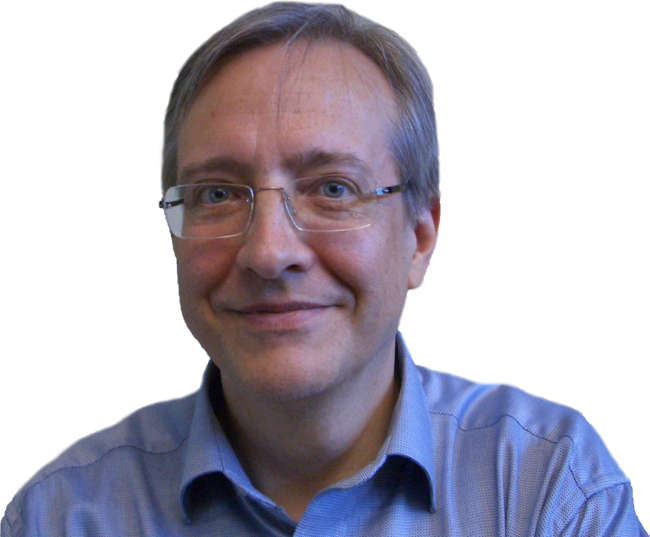
\includegraphics[width=0.8\linewidth]{bilder/dozenten/marten_frei.png}\\
\textit{Dr. Wolfgang Marten}

Hier geht es um Vektoren und Matrizen, sowie ein wenig Gruppentheorie.
Die "Ubungen sind zwar nicht immer einfach, geben aber einen sehr guten Ausblick auf die Klausur.

\subsubsection{Diskrete Mathematik}

% \begin{figure}[h]
% 	\centering\includegraphics[width=0.7\linewidth]{bilder/kemnitz.png}\\
% 	{Dr. Arnfried Kemnitz}
% \end{figure}
Diskrete Mathematik handelt von allem, was mit ganzen Zahlen zu tun hat: Fibbonacci-Zahlen, Primzahlen, Modulorechnung, usw.
Die Veranstaltung wird von Dr. Arnfried Kemnitz gehalten (leider kein Foto).


\subsubsection{Wissenschaftliches Arbeiten}

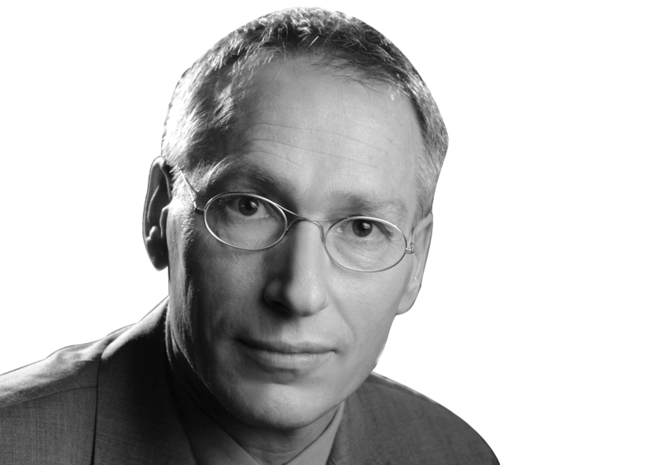
\includegraphics[width=0.9\linewidth]{bilder/dozenten/jung_frei.png}\\
\textit{Prof. Helmut Jung}

In dem Kurs "`wissenschaftliches Arbeiten"' lernen die Teilnehmer/-innen, Schritt f"ur Schritt eine wissenschaftliche Arbeit durchzuf"uhren -- beispielsweise eine Bachelorarbeit.
Hierzu erfahrt ihr, wie man systematisch vorgeht und welche Methoden
man in welchem Schritt verwenden kann. Er ist eine freiwillige
Schlüsselqualifikation, die Teilnahme wird aber empfohlen.
%Die Veranstaltung findet in zwei Gruppen statt, eine bei Prof. Jung und die andere bei Dr. Herrmann.
% Das gehört eigentlich nicht hier hin:

%Die Veranstaltung wird in zwei Gruppen angeboten: Der erste Kurs bei Prof. Jung findet Montag von 9:45 bis 11:15 Uhr und Dienstag von 11:30 bis 14:45 Uhr statt.
%Der zweite Kurs bei Dr. Herrmann findet Dienstag von 15:00 bis 16:30 Uhr statt.
%Beide Kurs haben denselben Inhalt und dieselbe Stundenzahl.
%Der zweite Kurs dauert das gesamte Semester, der andere endet entsprechend fr"uher.
\subsection{Interview mit PD Dr. Bode}

Privatdozent Dr. Bode leitet die großen und kleinen Übungen zur
Vorlesung ,,Diskrete Mathematik für Informatiker''. Er hat sich
freundlicherweise für ein Interview zur Verfügung gestellt.

\nquestion{Was und wo haben Sie studiert?} \\
Ich habe hier an der Technischen Universität Mathematik mit Nebenfach
Informatik studiert. Neben dem Diplom in Mathe habe ich dazu noch das
Vordiplom in Informatik gemacht.
\nquestion{Welchen Bezug haben Sie als Mathematiker zu Informatik?}\\
Für mich sind Computer in erster Linie ein Werkzeug, um bestimmte
mathematische Probleme zu lösen. Im Studium habe ich dazu
hauptsächlich Vorlesungen aus der theoretischen Informatik
gehört. Daneben habe ich als studentische Hilfskraft die Vorlesungen
,,Theoretische Informatik 1/2'' betreut.
%\nquestion{Erzählen Sie eine kleine Anekdote aus Ihrem Studium!}\\
\nquestion{Worum geht es in der Veranstaltung ,,Diskrete Mathematik für
Informatiker''?}\\
Sie behandelt wichtige Grundlagen, die die Studierenden später
brauchen werden. Inhaltlich geht es zunächst um allgemeine Grundlagen,
bevor wir uns etwas Kombinatorik, Zahlentheorie und Algebra angucken. \\
\nquestion{Welche Rolle spielen dabei die Übungen?}\\
Nun, die Übungen sind eine Ergänzung zur Vorlesung, die beim
Verständnis helfen sollen. Dazu sind sie eine gute Vorbereitung für
die Klausur. Dies klappt aber nur bei aktiver Mitarbeit der
Studierenden. Man sollte sich die Aufgaben schon vorher mal angeguckt
haben, sonst bringt das nichts. \footnote{Anmerkung des Interviewers:
Das kann ich aus eigener Erfahrung bestätigen, auch wenn man dabei
noch nichts versteht :)}. Die Meisten verhalten sich leider am Anfang
sehr passiv.\\
\nquestion{Was können Sie den Studierenden für das erste Semester mit
auf den Weg geben?}\\
Sie sollten  nicht alles glauben, was man ihnen
erzählt. Letztes Jahr gab es das Gerücht, dass die 1. große Übung
ausfällt, da es ja noch keine Vorlesung gab. Dem war nicht so, wir
haben da die Übungseinteilung gemacht. Da weniger anwesend waren, gab
es am Ende nicht so viele Übungen, wie man eigentlich gebraucht
hätte. Im Zweifelsfall gilt die Webseite zur Übung
\nurl{http://www.mathematik.tu-bs.de/jpbode/dm/}. Dort werden auch die
Übungsblätter veröffentlich.\\
Neben diesen speziellen Ratschlag noch einen Allgemeinen: Niemand wird
dafür umgebracht, Fragen zu stellen. Wenn also etwas unklar ist, nur
Mut!\\
\nquestion{Vielen Dank für das Interview!}\\
Bitte sehr. Zum Abschluss möchte ich allen Erstsemestern noch viel
Spaß und Erfolg im Studium wünschen.

